%\thispagestyle{intro}

% \section*{Conventions}
% \phantomsection
% \addcontentsline{toc}{section}{\protect\numberline{}Conventions}
\invisibleunnumberedchapter{Conventions}%

\begin{e1}
	\item Organisation du document:

	{\Large Chapitre} {\large Section} Sous-section {\small Sous-sous-section}

	\item Organisation des paragraphes:

	{\Large a} . {\large 1} . (a) . {\small (1)}
	
	\item Lien cliquable interne en \textcolor{\intlink}{gris}:
	
	\fullref{preparation}
	
	\item Lien cliquable externe en \textcolor{\extlink}{bleu}:
	
	\thirdwing

	\item Exemple tiré du \jp{}:

	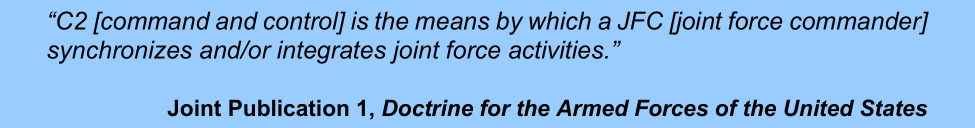
\includegraphics[width=0.7\paperwidth]{jptextex.png}

	\item Image tirée d'une publication Joint:

	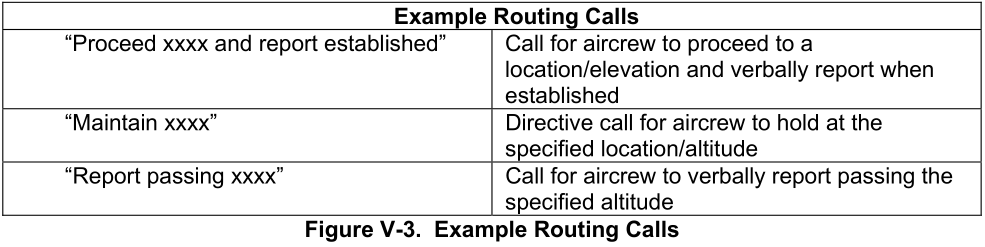
\includegraphics[width=0.7\paperwidth]{routing.png}
	
	Remarque: une image \emph{sans} source citée est tirée tu \jp{}; si une image provient d'une autre source, cette source sera citée sous l'image.

	\item Exemple:
	\begin{lstlisting}
		Sochi sol, REDWOLF, pour la mise en route
		REWOLF, Sochi sol, QNH 0758, vent calme, mise en route approuv"é"e, rappelez pr"ê"t "à" rouler}
	\end{lstlisting}

	\item \textbf{Emphase forte.}

	\item \emph{Emphase légère.}

	\item \important{Information importante.}
	
	%\item \useful{Information utile.}
	
	\item \remark{Remarque ou ensemble cohérent.}

	\item \note{Note de l'auteur. Contenu, suggestion ou opinion qui n'est pas extrait du \jp{}.}
	
	\item Mises à jour:
	
	\href{\latest}{Cliquez ici pour obtenir la dernière version de ce document.}

\end{e1} 